\documentclass{article}
\usepackage[top=2cm,bottom=2cm,left=2cm,right=2cm]{geometry}
\usepackage{CJKutf8}
\usepackage[dvipdfmx,unicode=true,colorlinks=false,pdfborder={0 0 0}]{hyperref}
\usepackage{indentfirst}
\usepackage[dvipdfmx]{graphicx}
\begin{document}
\begin{CJK}{UTF8}{gbsn}
\title{~\\[3cm]Zby's Printing Service\\石头、剪子、布 打印店\\使用说明 v0.1}
\author{北京大学附属中学 2014 届 5 单元 3 班 张博洋}
\date{2012 年 8 月}
\maketitle
\thispagestyle{empty}
\newpage
\renewcommand\contentsname{目\quad 录}
\renewcommand\figurename{图}
\renewcommand\tablename{表}
\newcommand{\zwfs}[2]{\frac{\;#1\;}{\;#2\;}}
\tableofcontents
\thispagestyle{empty}
\newpage
\pagenumbering{arabic}
\CJKindent

\section{打印店简介}
	\subsection{综述}
		石头、剪子、布打印店位于北大附中内, 由 2014 届 5 单元 3 班张博洋创建. 提供``云打印''服务, 支持 PC, Mac, iPhone, iPad, iPod Touch 等设备.
		
	\subsection{使用流程}
		本打印店的服务完全由用户自助完成. 一次打印过程仅需 2 步.
		\begin{itemize}
			\item{通过自己的设备将要打印的文稿提交至服务器.}
			\item{使用网页浏览器完成付费, 并根据自己的需要选择文稿的输出地点.}
		\end{itemize}
	
	\subsection{付费方法}
		本打印店采用预付费机制, 用户需要到学校里的售卖点购买充值卡\footnote{关于如何购买充值卡, 请看第 \pageref{sec:faq} 页的第 \ref{sec:faq} 节.}, 并到打印店的网站进行充值\footnote{关于充值方法, 请看第 \pageref{sec:recharge} 页的第 \ref{sec:recharge} 节.}.
	\subsection{计费方法}
		本打印店的计费方法与众不同, 墨粉与纸张分别单独计费, 具体来说是以下三点.
		\begin{itemize}
			\item{墨粉计费: 自动分析系统会分析出用户打印的文稿的页面黑色部分覆盖率, 以 5\% 为标准定价.}
			\item{纸张计费: 如果采用单面打印, 则纸张数即为页面数. 如果采用双面打印, 则纸张数为页面数的一半(上取整).}
			\item{计算公式: 设文档共有 $n$ 页, $f(i)$ 表示第 $i$ 页的页面覆盖率, $p$ 为墨粉单价, $q$ 为纸张单价, $s_1$ 为墨粉费用, $s_2$ 为纸张费用, $s$ 为总费用, 则计算公式如下:
				\begin{eqnarray}
					s_1 & = & \left[\sum_{i=1}^n \zwfs{f(i)}{5\%} \times p\right] \\[6pt]
					s_2 & = & \left\{
								\begin{array}{ll}
								\displaystyle nq, & \mbox{单面打印} \\[6pt]
								\displaystyle\left\lceil\zwfs{n}{2}\right\rceil q, & \mbox{双面打印}
								\end{array}
								\right. \\[6pt]
					s   & = & s_1 + s_2
				\end{eqnarray}
				
			}
		\end{itemize}
				
\newpage
\section{使用说明}
	\subsection{首次配置}
		\subsubsection{综述}
			如果您是第一次使用本打印店的服务, 您需要完成以下操作:
			\begin{itemize}
				\item{在自己的设备上配置好系统设置}
				\item{通过网页浏览器注册一个帐号.}
				\item{购买一张充值卡, 并通过网页浏览器充值.}
			\end{itemize}
		
		\subsubsection{配置系统设置}
			如果您使用的是学校的计算机, 则不需要进行此步骤, 学校的计算机已经安装好了软件.
			\paragraph{Microsoft Windows XP, Vista, 7, 8 操作系统}
				(以下操作会在您计算机上安装一个虚拟打印机, 并在桌面上添加一个网页图标, 以后您可以通过这个图标便捷地打开打印店的网站, 进行账户管理及文稿确认等操作.)
				\begin{itemize}
					\item{首先确认您拥有计算机的管理员权限, 然后使用电脑上的网页浏览器访问这个网址: \begin{verbatim}http://zby.pkuschool.edu.cn/\end{verbatim}}
					\item{根据网页上的提示, 下载好适用于 Microsoft Windows 的安装程序, 并运行, 安装程序如图 \ref{fig:installer_win} 所示, 安装过程中您只需要看说明并按回车即可.}
				\end{itemize}
				
				\begin{figure}[hp]
					\centering
					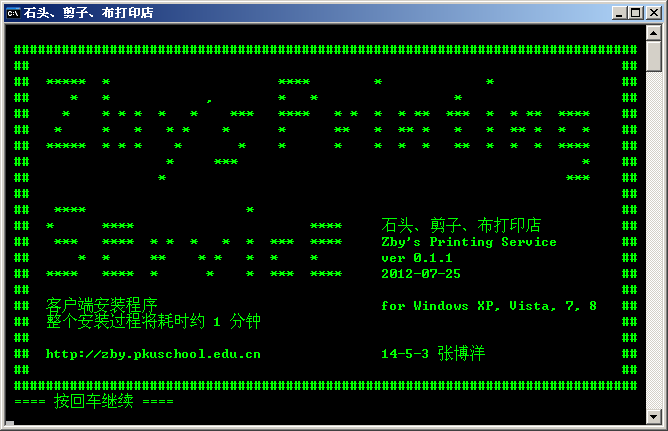
\includegraphics[height=0.45\textheight]{installer_win.png}
					\caption{在 Microsoft Windows 上的客户端安装程序}
					\label{fig:installer_win}
				\end{figure}
				\clearpage
			\paragraph{Mac OS X 操作系统}
				(以下操作会在您计算机上安装一个虚拟打印机, 并在``应用程序''中添加一个名为``Zby's Printing Service''的应用, 以后您可以通过这个应用便捷地打开打印店的网站, 进行账户管理及文稿确认等操作.)
				\begin{itemize}
					\item{首先确认您拥有计算机的管理员权限, 然后使用电脑上的网页浏览器访问这个网址: \begin{verbatim}http://zby.pkuschool.edu.cn/\end{verbatim}}
					\item{根据网页上的提示, 下载好适用于 Mac OS X 的安装器, 并运行, 安装程序如图 \ref{fig:installer_mac} 所示, 安装过程中您只需要看说明并按指示操作即可.}
				\end{itemize}
				
				\begin{figure}[hp]
					\centering
					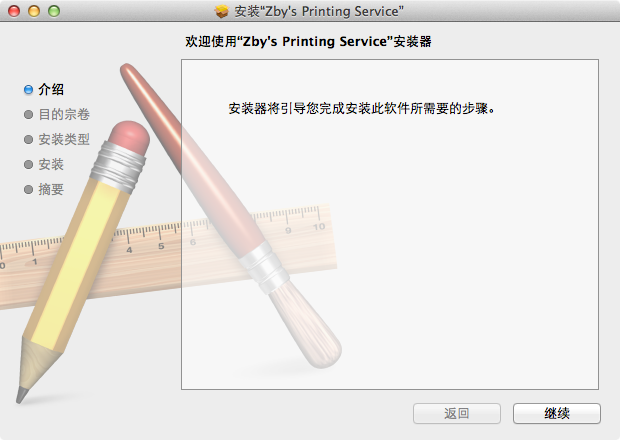
\includegraphics[height=0.45\textheight]{installer_mac.png}
					\caption{在 Mac OS X 上的客户端安装程序}
					\label{fig:installer_mac}
				\end{figure}
				\clearpage
			\paragraph{iPad, iPhone, iPod Touch 设备 (iOS 操作系统)}
				(以下操作会在您的设备上的主屏幕中添加一个网页图标, 以后您可以通过这个图标便捷地打开打印店的网站, 进行账户管理及文稿确认等操作.)
				\begin{itemize}
					\item{首先使用 Safari 网页浏览器访问这个网址: \begin{verbatim}http://zby.pkuschool.edu.cn/zbyprinting\end{verbatim}}
					\item{待页面完全打开后, 轻按工具栏中的那个发送形状的按钮, 在弹出的菜单中选择``添加至主屏幕'', 如图 \ref{fig:install_ipad1} 所示.}
					\item{在弹出的``添加至主屏幕''窗口中, 可以根据喜好编辑文本框内的内容, 作为主屏幕图标的名字, 如图 \ref{fig:install_ipad2} 所示.}
					\item{最后轻按``添加''便完成了.}
				\end{itemize}
				
				\begin{figure}[hp]
					\centering
					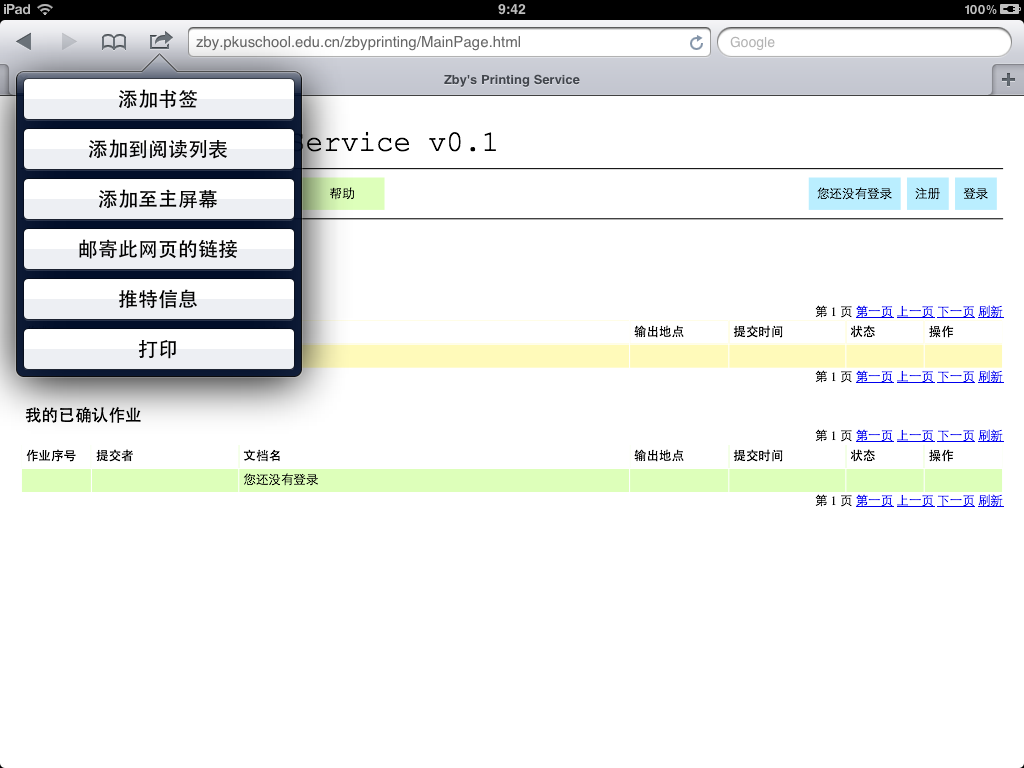
\includegraphics[height=0.45\textheight]{install_ipad1.png}
					\caption{在菜单中选择``添加至主屏幕''}
					\label{fig:install_ipad1}
				\end{figure}
				\begin{figure}[hp]
					\centering
					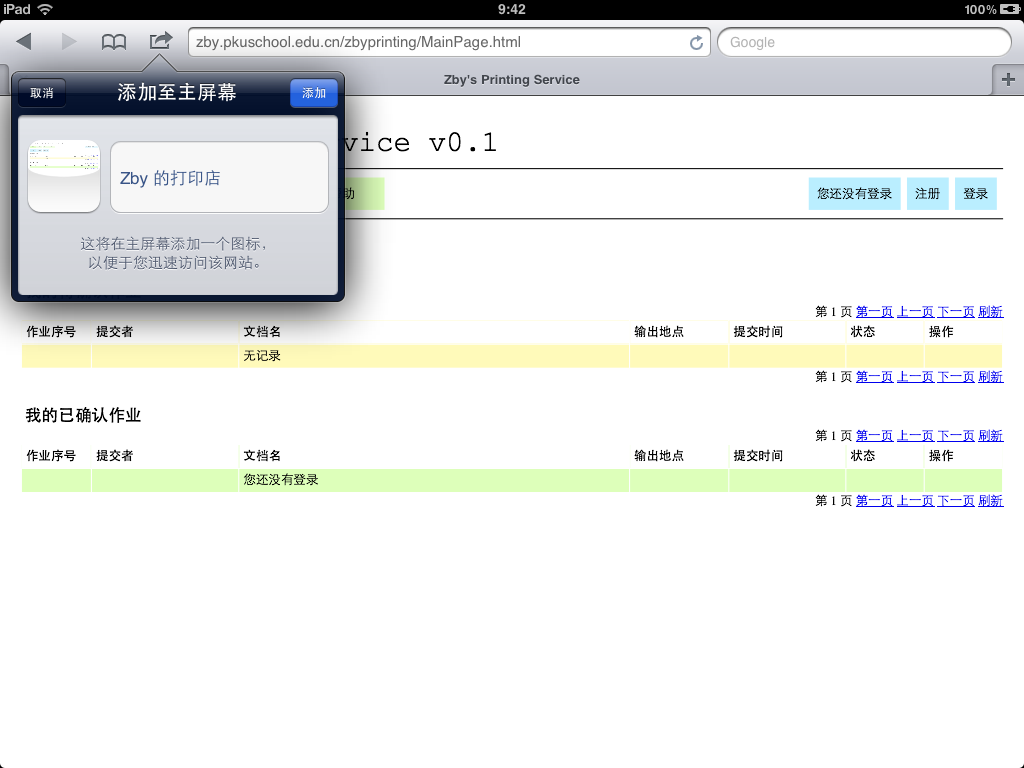
\includegraphics[height=0.45\textheight]{install_ipad2.png}
					\caption{``添加至主屏幕''窗口}
					\label{fig:install_ipad2}
				\end{figure}
				\clearpage
		
		\newpage
		\subsubsection{注册帐号并登录}
			\begin{itemize}
				\item{首先通过网页浏览器访问打印店的网站, 点击右上角的``注册''按钮, 如图 \ref{fig:register1} 所示.}
				\item{然后根据网页上的提示填好表格, 如图 \ref{fig:register2} 所示, 然后点击表单下方的``注册''按钮.}
				\item{如果一切顺利, 网页便会跳转至登录页面, 如图 \ref{fig:login} 所示, 在表单中填写好您的学号和密码, 然后点击登录.}
			\end{itemize}
			
			\begin{figure}[hp]
				\centering
				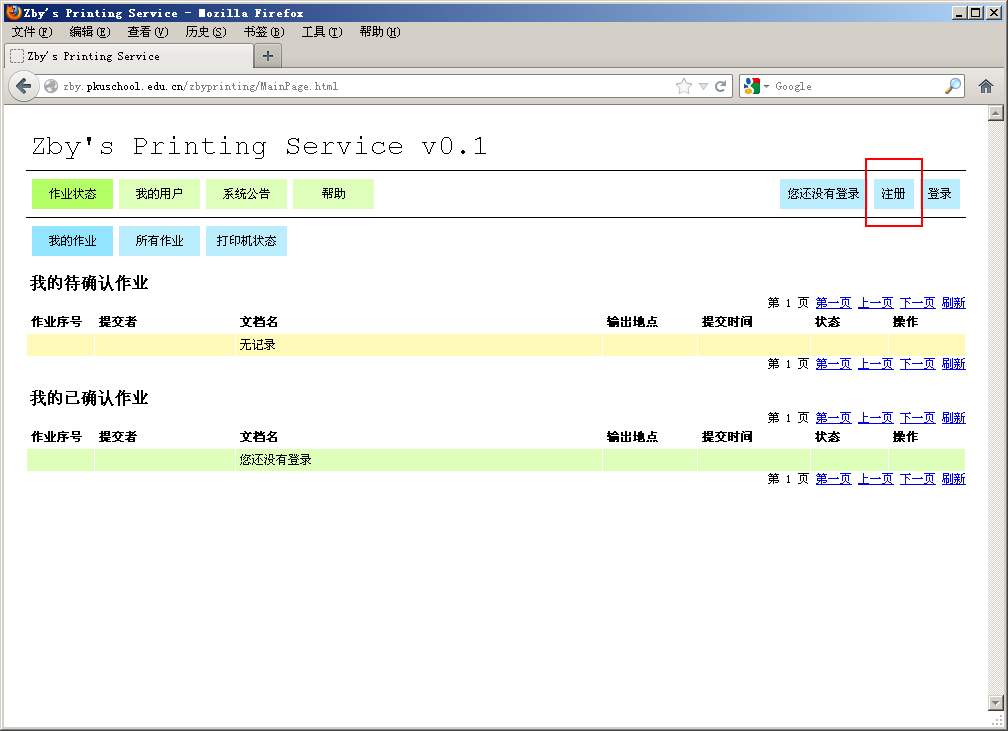
\includegraphics[height=0.45\textheight]{register1.png}
				\caption{点击右上角的``注册''按钮}
				\label{fig:register1}
			\end{figure}
			\begin{figure}[hp]
				\centering
				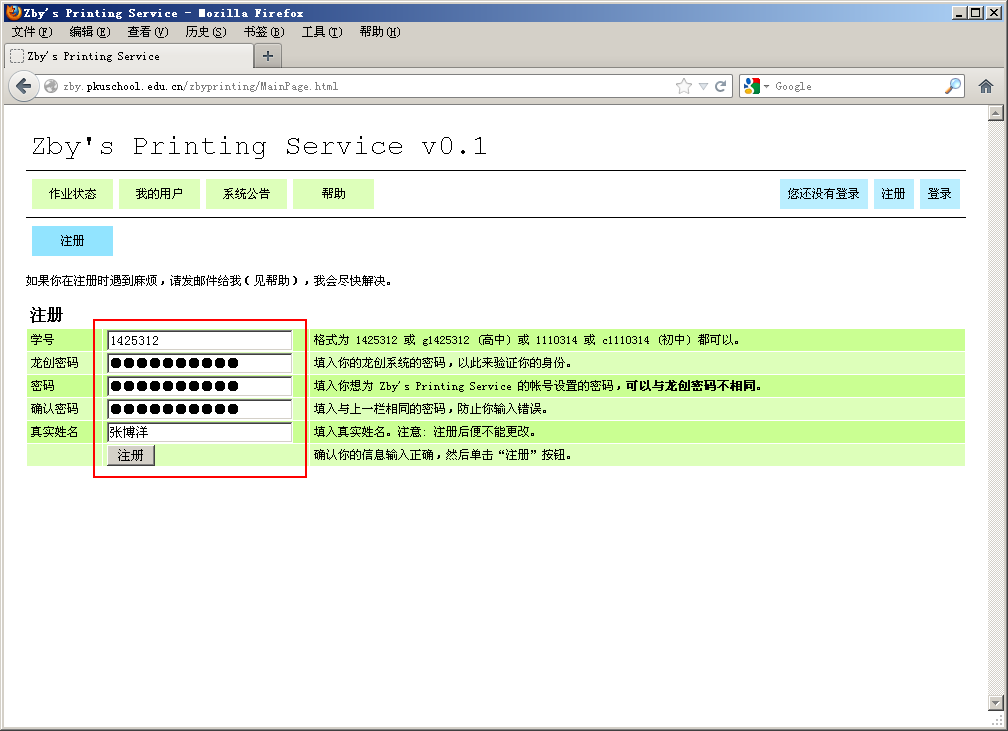
\includegraphics[height=0.45\textheight]{register2.png}
				\caption{填写注册表单}
				\label{fig:register2}
			\end{figure}
			\begin{figure}[hp]
				\centering
				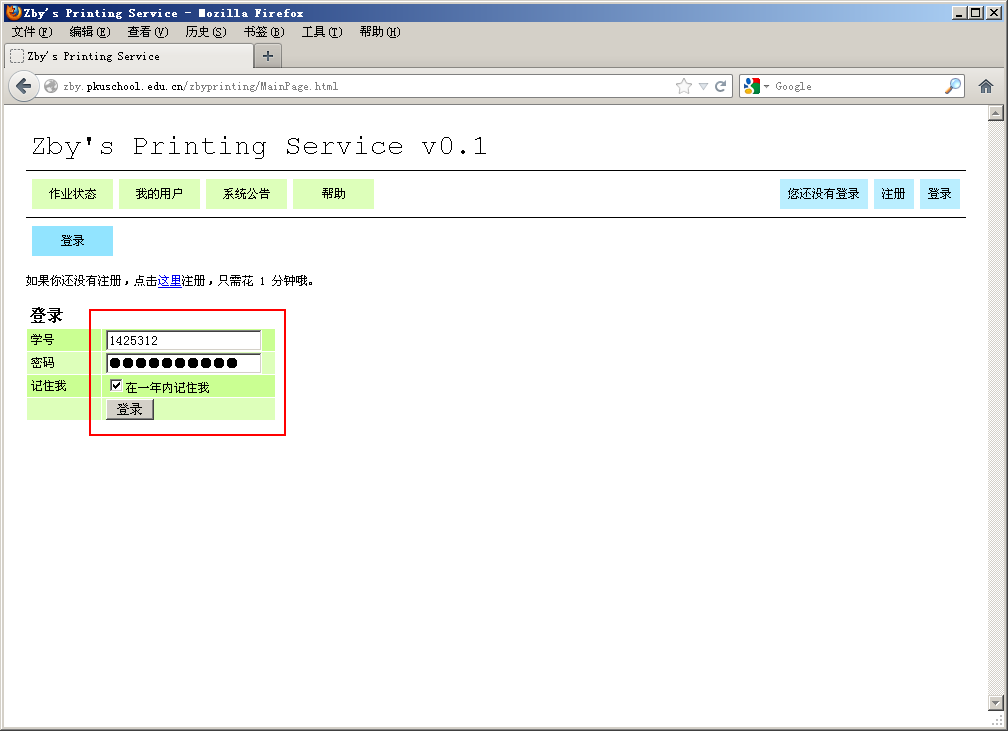
\includegraphics[height=0.45\textheight]{login.png}
				\caption{填写登录表单}
				\label{fig:login}
			\end{figure}
			\clearpage
		\subsubsection{为帐号充值}
			\label{sec:recharge}
			\begin{itemize}
				\item{首先确认您已经购买好了充值卡, 并已经登录了打印店的网站, 然后在主页上点击``我的用户'', 打开的网页如图 \ref{fig:recharge} 所示.}
				\item{在充值表单中填入 20 位的充值密码, 然后点击``充值''按钮. 如果一切顺利, 网页将会刷新, 在``账户余额''中便会显示新的余额.}
			\end{itemize}
			
			\begin{figure}[hp]
				\centering
				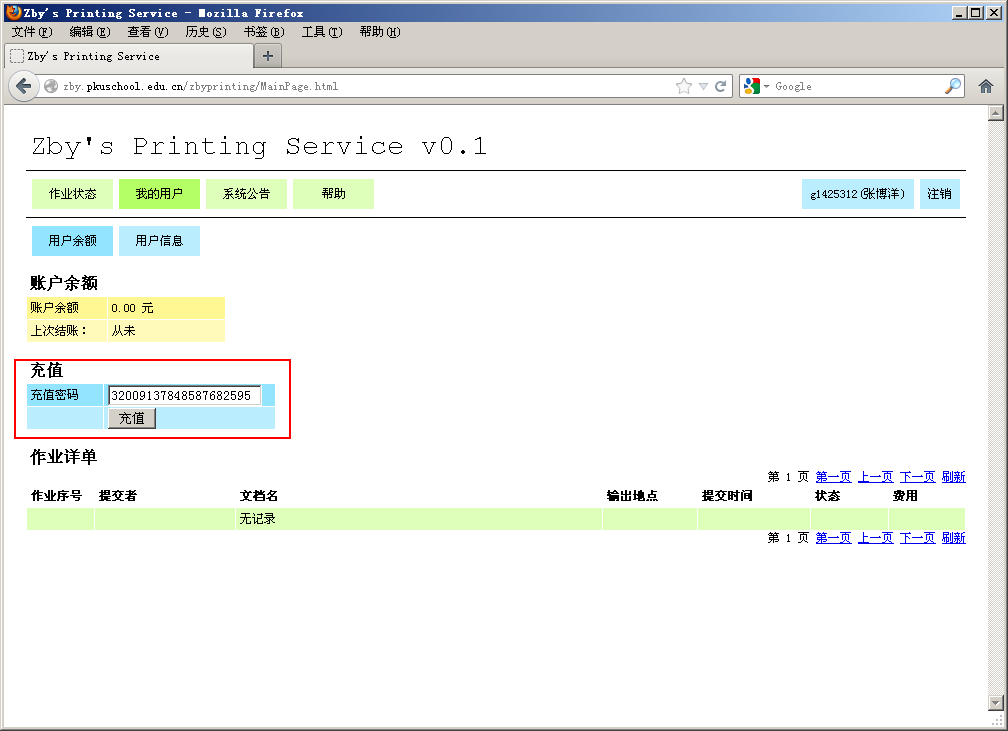
\includegraphics[height=0.45\textheight]{recharge.png}
				\caption{填写 20 位充值密码}
				\label{fig:recharge}
			\end{figure}
			\clearpage
	\newpage
	\subsection{打印文稿}
		打印一篇文稿仅需以下 2 步.
		\begin{itemize}
			\item{通过自己的设备将要打印的文稿提交至服务器.}
			\item{使用网页浏览器根据自己的需要修改打印设置.}
		\end{itemize}
		
		\subsubsection{将文稿提交至服务器}
			将文稿提交至服务器十分简单, 仅需要按照普通的打印流程, 在选择打印机的时候选择打印店的打印机即可.
			\paragraph{Microsoft Windows XP, Vista, 7, 8 操作系统}
				(这里以 Microsoft Word 2007 为例)
				\begin{itemize}
					\item{与在本地打印机上打印一样, 选择 Word 菜单中的``打印''\footnote{如果您的计算机上之前没有安装过打印机, 或者您已经将``Zby's Printing Service''设置为了默认打印机, 您可以直接选择快速打印, 无须调整任何设置.}, 如图 \ref{fig:word_win} 所示.}
					\item{在弹出的窗口中, 在``打印机''一栏里选择 ``Zby's Printing Service'', 不要更改其他设置, 如图 \ref{fig:print_win} 所示. 然后点击``确定''即可.}
				\end{itemize}
				
				\begin{figure}[hp]
					\centering
					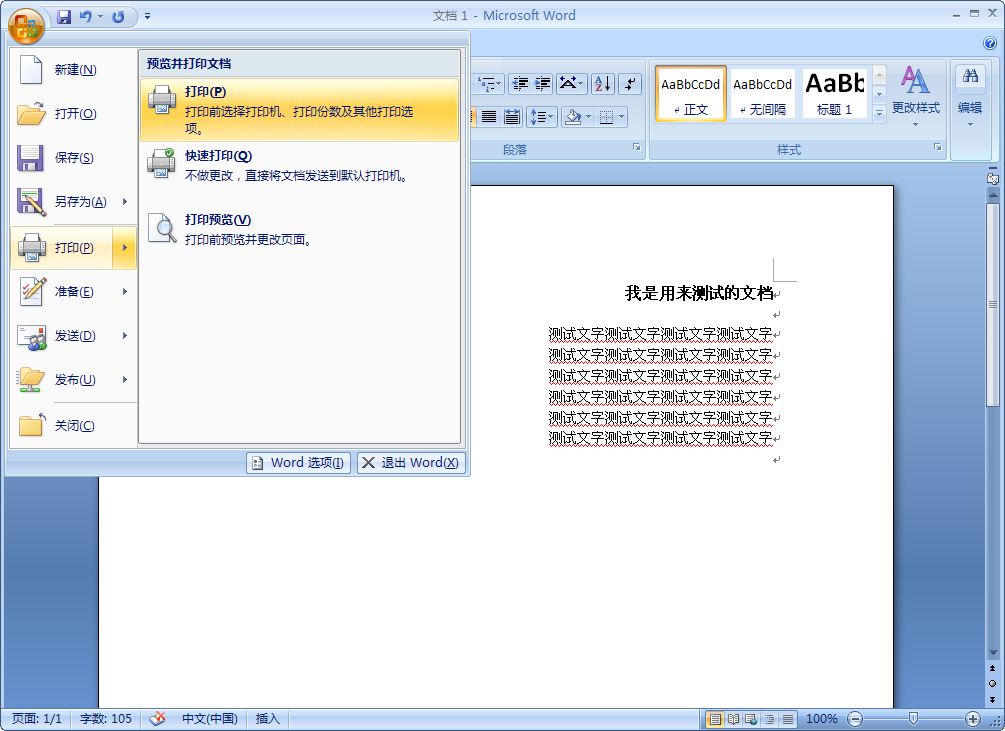
\includegraphics[height=0.45\textheight]{word_win.png}
					\caption{选择 Word 菜单中的``打印''}
					\label{fig:word_win}
				\end{figure}
				\begin{figure}[hp]
					\centering
					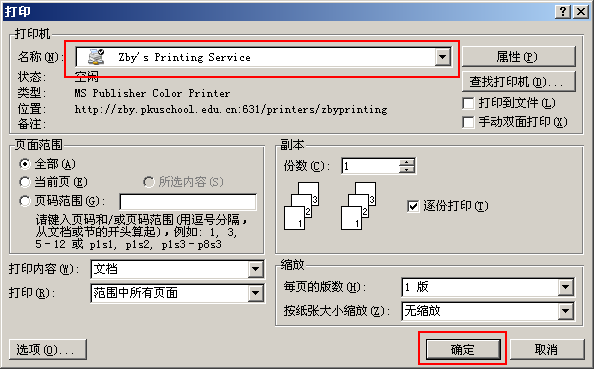
\includegraphics[height=0.45\textheight]{print_win.png}
					\caption{``打印''选项窗口}
					\label{fig:print_win}
				\end{figure}
				\clearpage
				
			\paragraph{Mac OS X 操作系统}
				(这里以 Microsoft Word for Mac 2011 为例)
				\begin{itemize}
					\item{与在本地打印机上打印一样, 选择 Word ``文件''菜单中的``打印''\footnote{如果您的计算机上之前没有安装过打印机, 或者您已经将``石头、剪子、布 打印店''设置为了默认打印机, 您可以直接选择工具栏中的快速打印, 无须调整任何设置.}, 如图 \ref{fig:word_mac} 所示.}
					\item{在弹出的窗口中, 在``打印机''一栏里选择 ``石头、剪子、布 打印店'', 不要更改其他设置, 如图 \ref{fig:print_mac} 所示. 然后点击``确定''即可.}
				\end{itemize}
				
				\begin{figure}[hp]
					\centering
					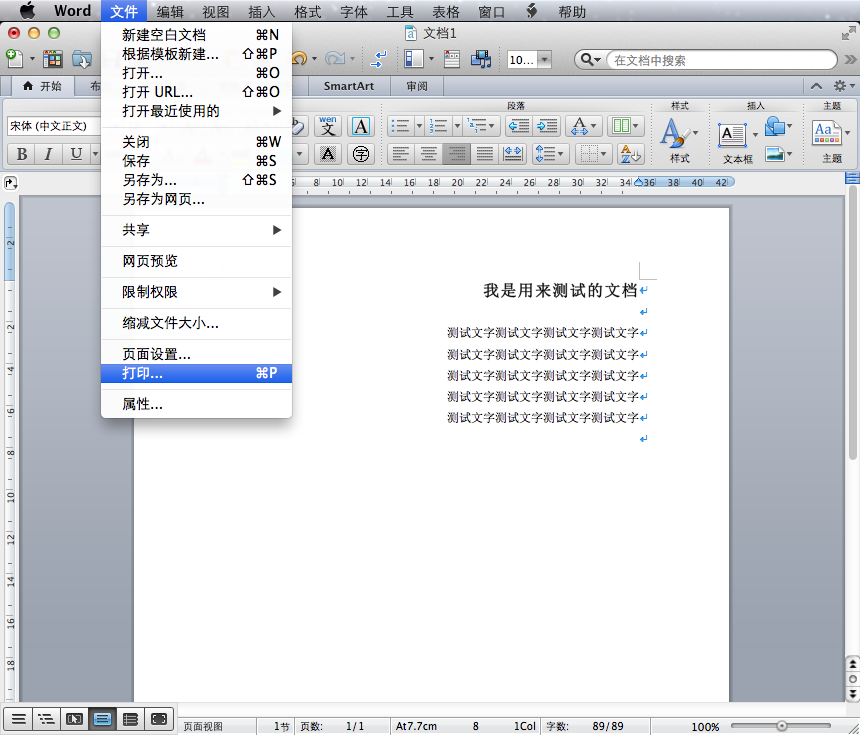
\includegraphics[height=0.45\textheight]{word_mac.png}
					\caption{选择 Word 菜单中的``打印''}
					\label{fig:word_mac}
				\end{figure}
				\begin{figure}[hp]
					\centering
					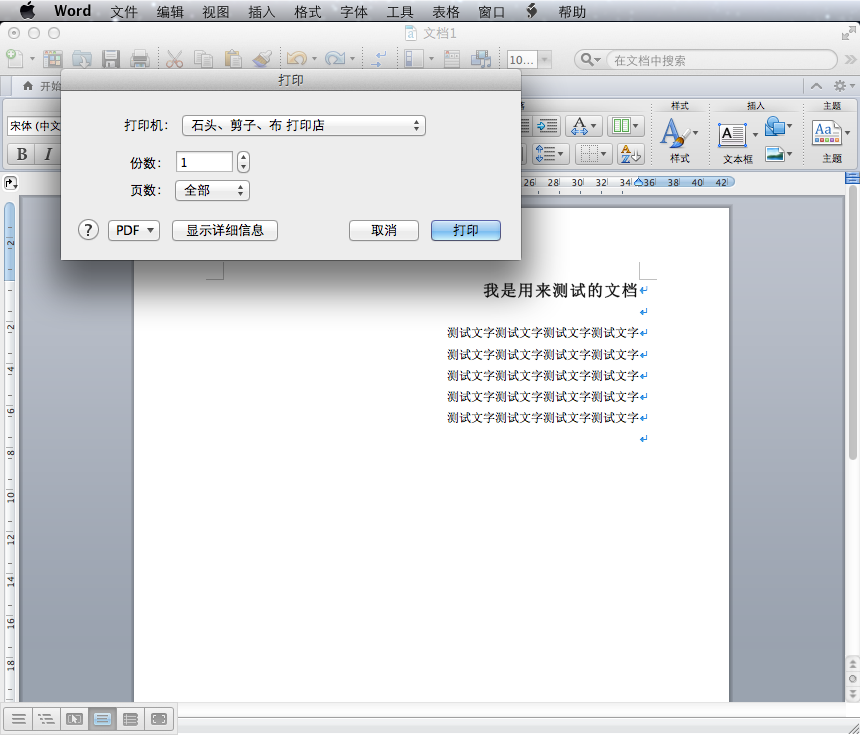
\includegraphics[height=0.45\textheight]{print_mac.png}
					\caption{``打印''选项窗口}
					\label{fig:print_mac}
				\end{figure}
				\clearpage
				
			\paragraph{iPad, iPhone, iPod Touch 设备 (iOS 操作系统)}
				(这里以使用 Safari 网页浏览器\footnote{只要是支持 AirPrint 技术的应用软件都可以, 例如 Safari, Mail, iBook 等.}打印网页为例)
				\begin{itemize}
					\item{打开 Safari 网页浏览器, 轻按工具栏中的那个发送形状的按钮, 在弹出的菜单中选择``打印'', 如图 \ref{fig:print_ipad1} 所示.}
					\item{在弹出的``打印机选项''窗口中, 在``打印机''一栏中选择 ``剪刀、石头、布打印店'', 不要改动其他设置, 如图 \ref{fig:print_ipad2} 所示. 然后轻按``打印''即可.}
				\end{itemize}
				
				\begin{figure}[hp]
					\centering
					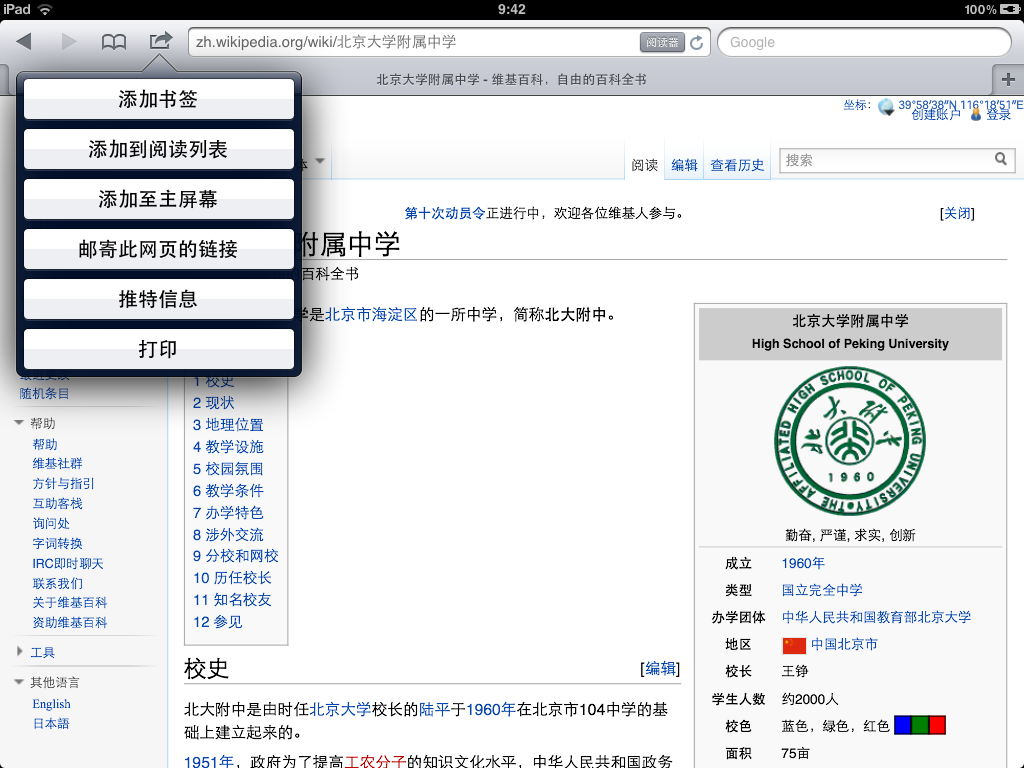
\includegraphics[height=0.45\textheight]{print_ipad1.png}
					\caption{从菜单中选择``打印''}
					\label{fig:print_ipad1}
				\end{figure}
				\begin{figure}[hp]
					\centering
					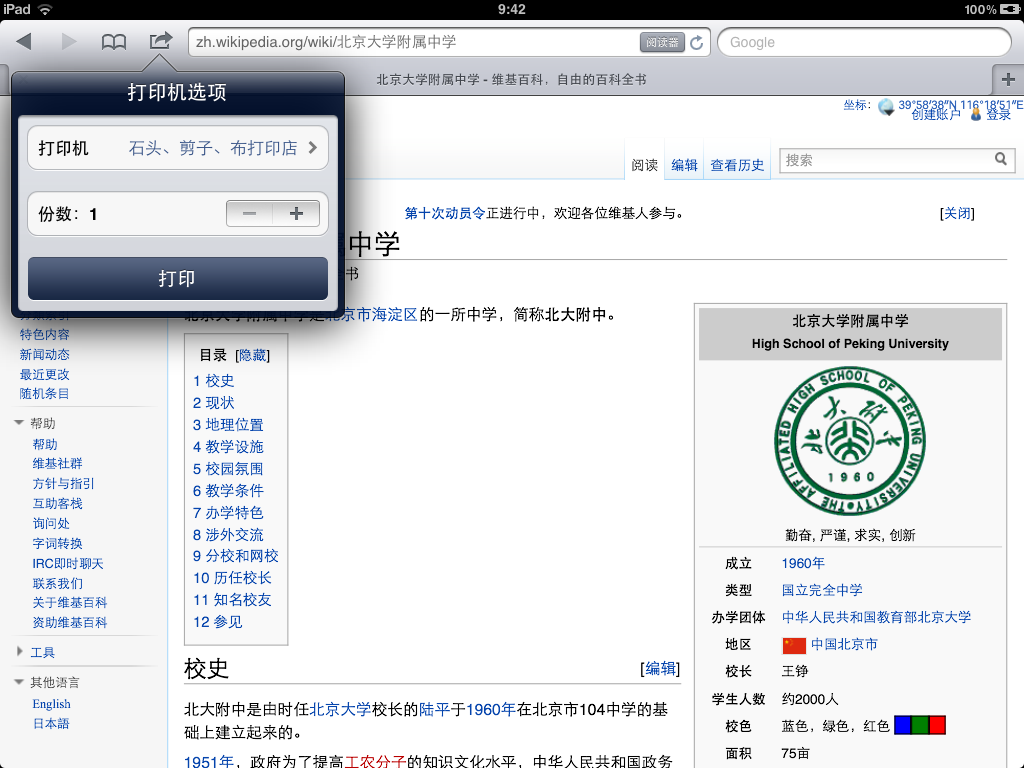
\includegraphics[height=0.45\textheight]{print_ipad2.png}
					\caption{``打印机''一栏中选择 ``剪刀、石头、布打印店''}
					\label{fig:print_ipad2}
				\end{figure}
				\clearpage
		\newpage
		\subsubsection{修改打印设置}
			\begin{itemize}
				\item{首先通过网页浏览器访问打印店的网站, 如果您还没有登录, 请先登录. 刚才提交的文稿将会在``我的待确认作业''一栏中显示. 如果没有显示出来, 请点击表格右上角的``刷新''按钮, 如图 \ref{fig:jobconfirm1} 所示.}
				\item{点击``操作''一栏中的``确认''按钮, 网页将会跳转到确认页面, 在这个页面中, 您可以查看页面覆盖率分析结果, 选择输出的地点, 是否需要双面打印, 如图 \ref{fig:jobconfirm2} 所示.}
				\item{选择完毕后, 点击最下方的``提交''按钮, 系统将会为您开始打印, 页面会跳转至主页, 开始打印的文稿将会出现在``我的已确认作业''中, 如图 \ref{fig:jobconfirm3} 所示.}
			\end{itemize}
			
			\begin{figure}[hp]
				\centering
				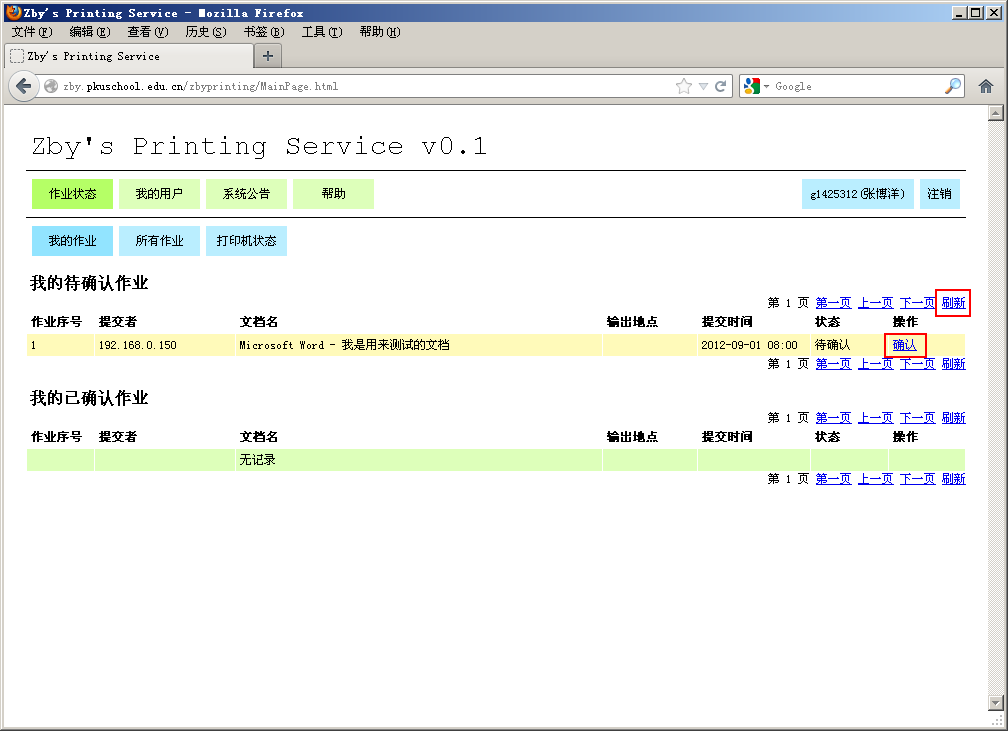
\includegraphics[height=0.45\textheight]{jobconfirm1.png}
				\caption{``我的待确认作业''中刚提交的作业}
				\label{fig:jobconfirm1}
			\end{figure}
			\begin{figure}[hp]
				\centering
				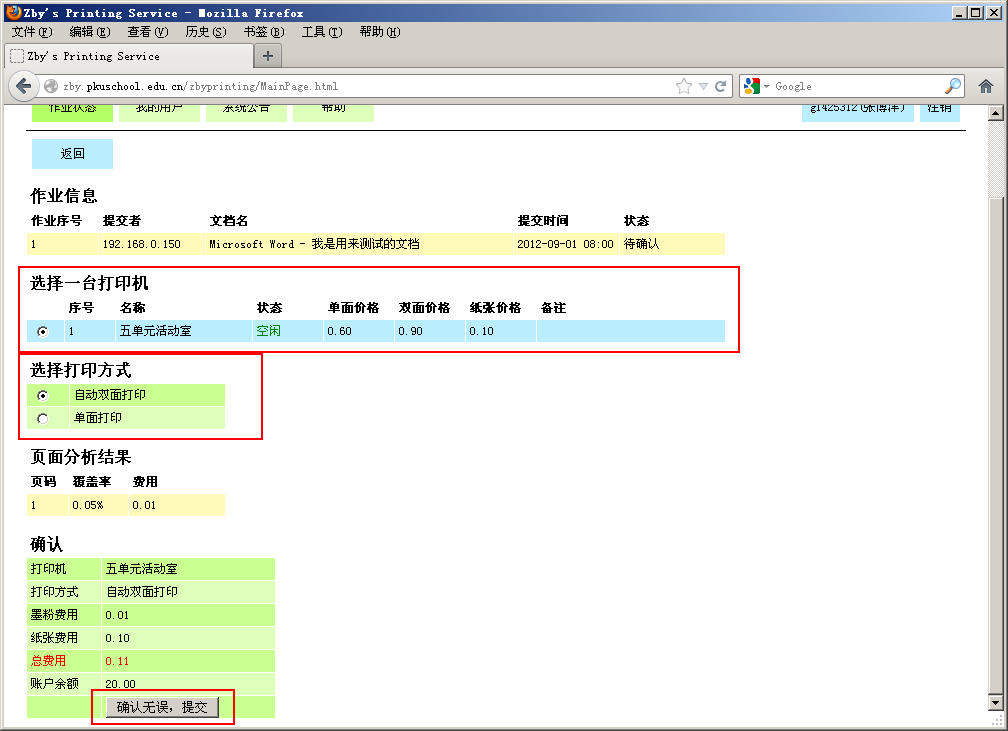
\includegraphics[height=0.45\textheight]{jobconfirm2.png}
				\caption{作业确认页面}
				\label{fig:jobconfirm2}
			\end{figure}
			\begin{figure}[hp]
				\centering
				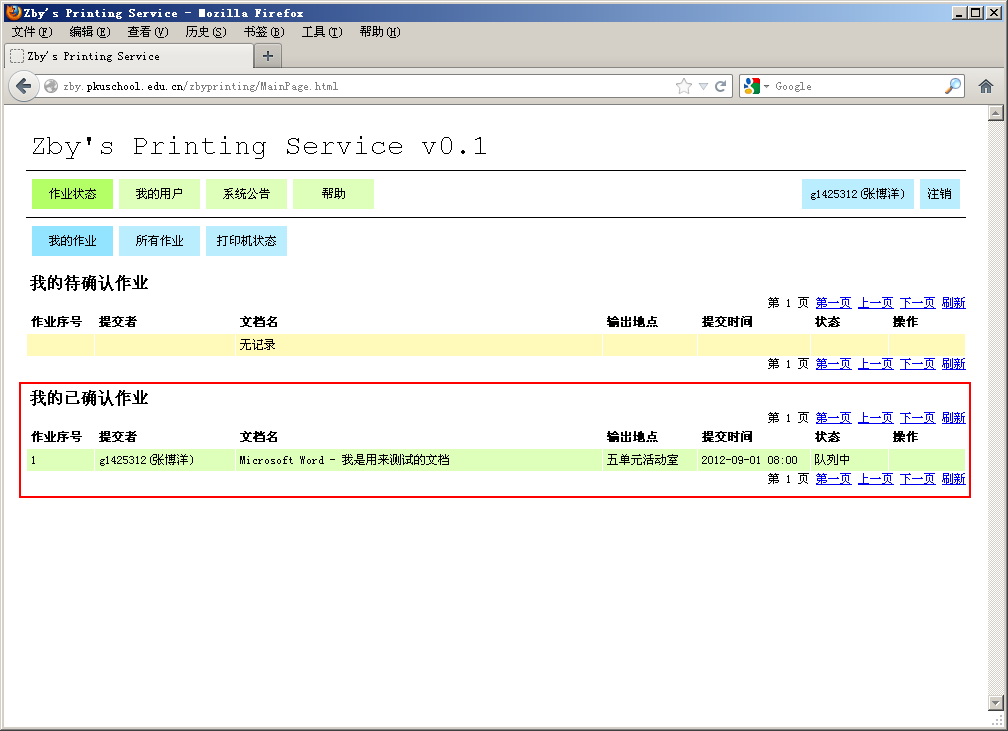
\includegraphics[height=0.45\textheight]{jobconfirm3.png}
				\caption{``我的已确认作业''中刚确认的作业}
				\label{fig:jobconfirm3}
			\end{figure}
			\clearpage

\newpage
\section{常见问题及解答}
	\subsection{常见问题及解答}
		\label{sec:faq}
		这里集合了打印店的常见问题, 如果这没能解决您的问题, 请联系我.
		\begin{itemize}
			\item{\textbf{我去哪里购买充值卡?}
			
				关于充值卡的购买信息, 请看下面网址上的信息.
				\begin{verbatim}
					http://page.renren.com/601487471/note/869116543
					http://zby.no-ip.org/wordpress/?p=333
				\end{verbatim}
			}
			\item{\textbf{打印店主页中的``作业''是什么意思?}
			
				这个``作业''其实是``job''的意思, 对于服务器来说就是``打印作业''.
			}
			\item{\textbf{错误: 网页提示``操作超时''.}
				
				这是由于您提交作业后 15 分钟内没有及时确认作业, 系统自动取消作业造成的. 您可以再提交一遍, 并在 15 分钟内完成作业确认.
			}
			\item{\textbf{错误: 网页提示``纸张错误''.}
			
				这是由于您的文档采用的纸张不是标准的 A4 纸. 目前本打印店不提供除 A4 纸以外的纸张. 请调整您的纸张设置, 再试一次.
			}
			\item{\textbf{错误: 网页提示``已完成''但是文稿并没有打印出来.}
			
				这可能是由于打印机或服务器出现问题. 请联系我, 在核实情况后我将进行退费等操作. 在此之前, 请更换一个输出地点再试一次.
			}
			\item{\textbf{错误: 我打不开打印店的网页.}
			
				首先请您确认您的网址是否正确, 是否以及接入北大附中的内网(通过 Wifi 等), 是否在服务时间内. 如果这些都正确无误, 那么有可能是服务器发生问题, 请稍候再试一次.
			}
			
		\end{itemize}
	
	\subsection{联系方式}	
		如果您在使用中有任何问题, 请发邮件至 \textit{zbyprinting@126.com} 或者访问下面的网址, 我将尽力回答您的问题.
		\begin{verbatim}
			http://page.renren.com/601487471
			http://zby.no-ip.org/wordpress/?cat=9
		\end{verbatim}
		
	\subsection{获取源代码}
		本打印店的软件为自由软件, 使用 LGPL 授权发布. 如果您需要源代码, 请从下面的地址获取.
		\begin{verbatim}
			git://zby.no-ip.org/zbyprinting
			http://zby.no-ip.org/gitweb/?p=zbyprinting;a=summary
		\end{verbatim}

\newpage
\end{CJK}
\end{document}
